% !TeX program = xelatex
\documentclass[UTF8,fontset=windows,12pt,a4paper]{ctexart}

\usepackage{geometry}
\usepackage{graphicx}
\usepackage{booktabs}
\usepackage{longtable}
\usepackage{tabularx}
\usepackage{array}
\usepackage{enumitem}
\usepackage{float}
\usepackage{placeins}
\usepackage{caption}
\usepackage{subcaption}
\usepackage{xcolor}
\usepackage{listings}
\usepackage{tikz}
\usepackage{hyperref}
\usepackage{fancyhdr}
\usepackage{setspace}

\usetikzlibrary{arrows.meta,positioning}
\graphicspath{{figures/}}

\geometry{left=2.58cm,right=2.58cm,top=2.54cm,bottom=2.54cm}
\setstretch{1.5}
\setlength{\parindent}{2em}
\setlength{\parskip}{0.2em}
\captionsetup{font=small,labelsep=space}
\hypersetup{
  colorlinks=true,
  linkcolor=black,
  urlcolor=blue,
  citecolor=black,
  pdfauthor={Troy},
  pdftitle={基于 STM32F103C8T6 的智能手表设计}
}

\pagestyle{fancy}
\fancyhf{}
\fancyhead[L]{嵌入式系统课程设计}
\fancyhead[R]{基于 STM32F103C8T6 的智能手表设计}
\fancyfoot[C]{\thepage}
\setlength{\headheight}{15pt}
\renewcommand{\headrulewidth}{0.4pt}

\lstdefinestyle{cstyle}{
  language=C,
  basicstyle=\small\ttfamily,
  keywordstyle=\color{blue!70!black}\bfseries,
  commentstyle=\color{green!40!black},
  stringstyle=\color{orange!70!black},
  numbers=left,
  numberstyle=\tiny\color{gray},
  frame=single,
  breaklines=true,
  columns=fullflexible,
  tabsize=4,
  showstringspaces=false
}

\newcolumntype{Y}{>{\raggedright\arraybackslash}X}

\begin{document}

\pagenumbering{gobble}
\begin{titlepage}
  \centering
  \vspace*{1.2cm}
  
\includegraphics[width=0.72\textwidth]{gdut.pdf}

  \vspace{2.2cm}
  {\zihao{1}\bfseries 嵌入式系统课程设计报告\par}

  \vspace{1.0cm}
  {\zihao{2}\bfseries 基于 STM32F103C8T6 的智能手表设计\par}

  \vspace{2.0cm}
  \renewcommand{\arraystretch}{1.6}
  \begin{tabular}{rl}
    姓名： & 叶楚轶 \\
    学号： & 3124007715 \\
    专业： & 微电子科学与工程 \\
    班级： & 4 \\
    指导教师： & 周贤中 \\
    完成日期： & \today \\
  \end{tabular}

  \vfill
  
\includegraphics[height=1.1cm]{gdut-integrated-horizontal.pdf}
\end{titlepage}

\newpage
\begin{abstract}
本文围绕嵌入式系统课程设计题目，设计并实现了一套基于 STM32F103C8T6 的智能手表原型系统。系统以 STM32F103C8T6 最小系统板为主控，使用 SSD1306 OLED 完成表盘和多页面信息显示，使用 MPU6050 采集姿态与加速度数据，使用旋转编码器和独立按键完成人机交互，使用 HC-05 蓝牙模块与 Android 手机上位机进行数据同步和远程控制。软件部分基于 STM32 HAL 与 FreeRTOS 实现多任务调度，将时钟维护、输入扫描、传感器采集、OLED 刷新和蓝牙通信拆分为独立任务，提高了系统结构的清晰度和可维护性。

本项目完成了 OLED 表盘显示、页面切换、MPU6050 数据读取、计步、蓝牙连接状态显示、手机同步时间、手机切换页面、清零步数、请求状态和查看传感器数据等功能。经教师确认，本课程设计可以不制作 PCB，因此本项目采用最小系统板和模块化接线完成实物验证，并将蓝牙上位机与计步功能作为扩展重点。

\textbf{关键词：} STM32F103C8T6；FreeRTOS；SSD1306；MPU6050；HC-05；Android 上位机；智能手表
\end{abstract}

\clearpage
\tableofcontents
\clearpage
\pagenumbering{arabic}
\setcounter{page}{1}

\section{项目简介}

\subsection{项目背景}

智能手表是典型的嵌入式综合应用场景，涉及低功耗微控制器、显示、人机交互、传感器采集、无线通信和上位机应用等多个模块。课程设计要求以 STM32F103C8T6 为核心完成一个可演示的智能手表原型，重点考察硬件连接、外设驱动、FreeRTOS 任务划分、模块协作和最终演示效果。

本项目在 STM32F103C8T6 最小系统板基础上搭建实物系统。由于教师已说明可以不制作 PCB，本设计未进行正式 PCB 打样，而是采用模块化硬件和杜邦线连接完成调试与验收。该方式更适合课程设计阶段的快速迭代，同时保留了后续绘制 PCB 的扩展空间。

\subsection{主要功能}

系统最终实现的功能包括：
\begin{itemize}[leftmargin=2em]
  \item OLED 主表盘显示时间、日期、电量图标、蓝牙状态和 IMU 状态；
  \item OLED 多页面显示，包含表盘页、IMU 数据页、计步页、蓝牙页和设备信息页；
  \item 旋转编码器切换页面，独立按键返回主表盘；
  \item MPU6050 读取加速度、角速度和姿态角，并基于加速度完成基础计步；
  \item HC-05 蓝牙模块通过 USART2 与手机通信；
  \item Android 上位机连接 HC-05 后，可同步时间、切换页面、清零步数、请求状态并查看传感器数据。
\end{itemize}

\section{项目设计目标}

\subsection{基本目标}

根据课程设计要求，本项目需要完成智能手表的基本显示与传感器功能。具体目标如下：
\begin{enumerate}[leftmargin=2em]
  \item 完成 STM32F103C8T6 最小系统板与 OLED、MPU6050、输入模块的硬件连接；
  \item 基于 FreeRTOS 完成多任务程序结构，避免所有逻辑堆叠在单一主循环中；
  \item 实现 OLED 时间页面和传感器页面，保证信息刷新稳定；
  \item 完成 MPU6050 初始化、在线检测和数据读取；
  \item 完成可现场演示的实物作品和配套说明文档。
\end{enumerate}

\subsection{扩展目标}

在基本目标之外，本项目进一步完成了以下扩展内容：
\begin{itemize}[leftmargin=2em]
  \item 增加旋转编码器，形成多页面交互；
  \item 增加 HC-05 蓝牙通信，实现与 Android 手机的数据同步；
  \item 设计 Android 蓝牙上位机，完成手机端控制与数据查看；
  \item 实现基础运动计步功能，并支持手机端清零；
  \item 不制作 PCB，改为使用最小系统板和模块化接线完成实物验证。
\end{itemize}

\section{项目设计与实现}

\subsection{系统总体架构}

系统由 STM32 主控、OLED 显示、MPU6050 传感器、输入模块、HC-05 蓝牙模块和 Android 上位机构成。总体结构如图~\ref{fig:system-arch} 所示。

\begin{figure}[H]
  \centering
  \resizebox{0.96\textwidth}{!}{%
  \begin{tikzpicture}[
    node distance=1.05cm and 1.15cm,
    block/.style={draw, rounded corners=2pt, align=center, minimum width=2.75cm, minimum height=0.9cm},
    arrow/.style={-{Latex[length=2mm]}, thick}
  ]
    \node[block, fill=blue!8] (mcu) {STM32F103C8T6\\FreeRTOS};
    \node[block, fill=green!8, above left=of mcu] (oled) {SSD1306 OLED\\I2C1};
    \node[block, fill=green!8, below left=of mcu] (mpu) {MPU6050\\I2C2};
    \node[block, fill=yellow!12, above right=of mcu] (input) {旋转编码器\\PB1 按键};
    \node[block, fill=orange!10, below right=of mcu] (bt) {HC-05 蓝牙\\USART2};
    \node[block, fill=purple!8, right=1.2cm of bt] (phone) {Android 上位机\\SPP 控制};

    \draw[arrow] (mcu) -- node[above, sloped]{显示刷新} (oled);
    \draw[arrow] (mpu) -- node[below, sloped]{传感器数据} (mcu);
    \draw[arrow] (input) -- node[above, sloped]{页面控制} (mcu);
    \draw[arrow] (mcu) -- node[above, sloped]{帧协议} (bt);
    \draw[arrow] (bt) -- node[above]{经典蓝牙} (phone);
  \end{tikzpicture}%
  }
  \caption{智能手表系统总体架构}
  \label{fig:system-arch}
\end{figure}

\subsection{硬件设计}

硬件采用模块化连接方式。实物接线效果如图~\ref{fig:hardware-wiring} 所示。所有模块必须共地，OLED 和 MPU6050 均使用 I2C 通信，但分别挂在 I2C1 与 I2C2，避免地址或总线时序互相影响。

\begin{figure}[H]
  \centering
  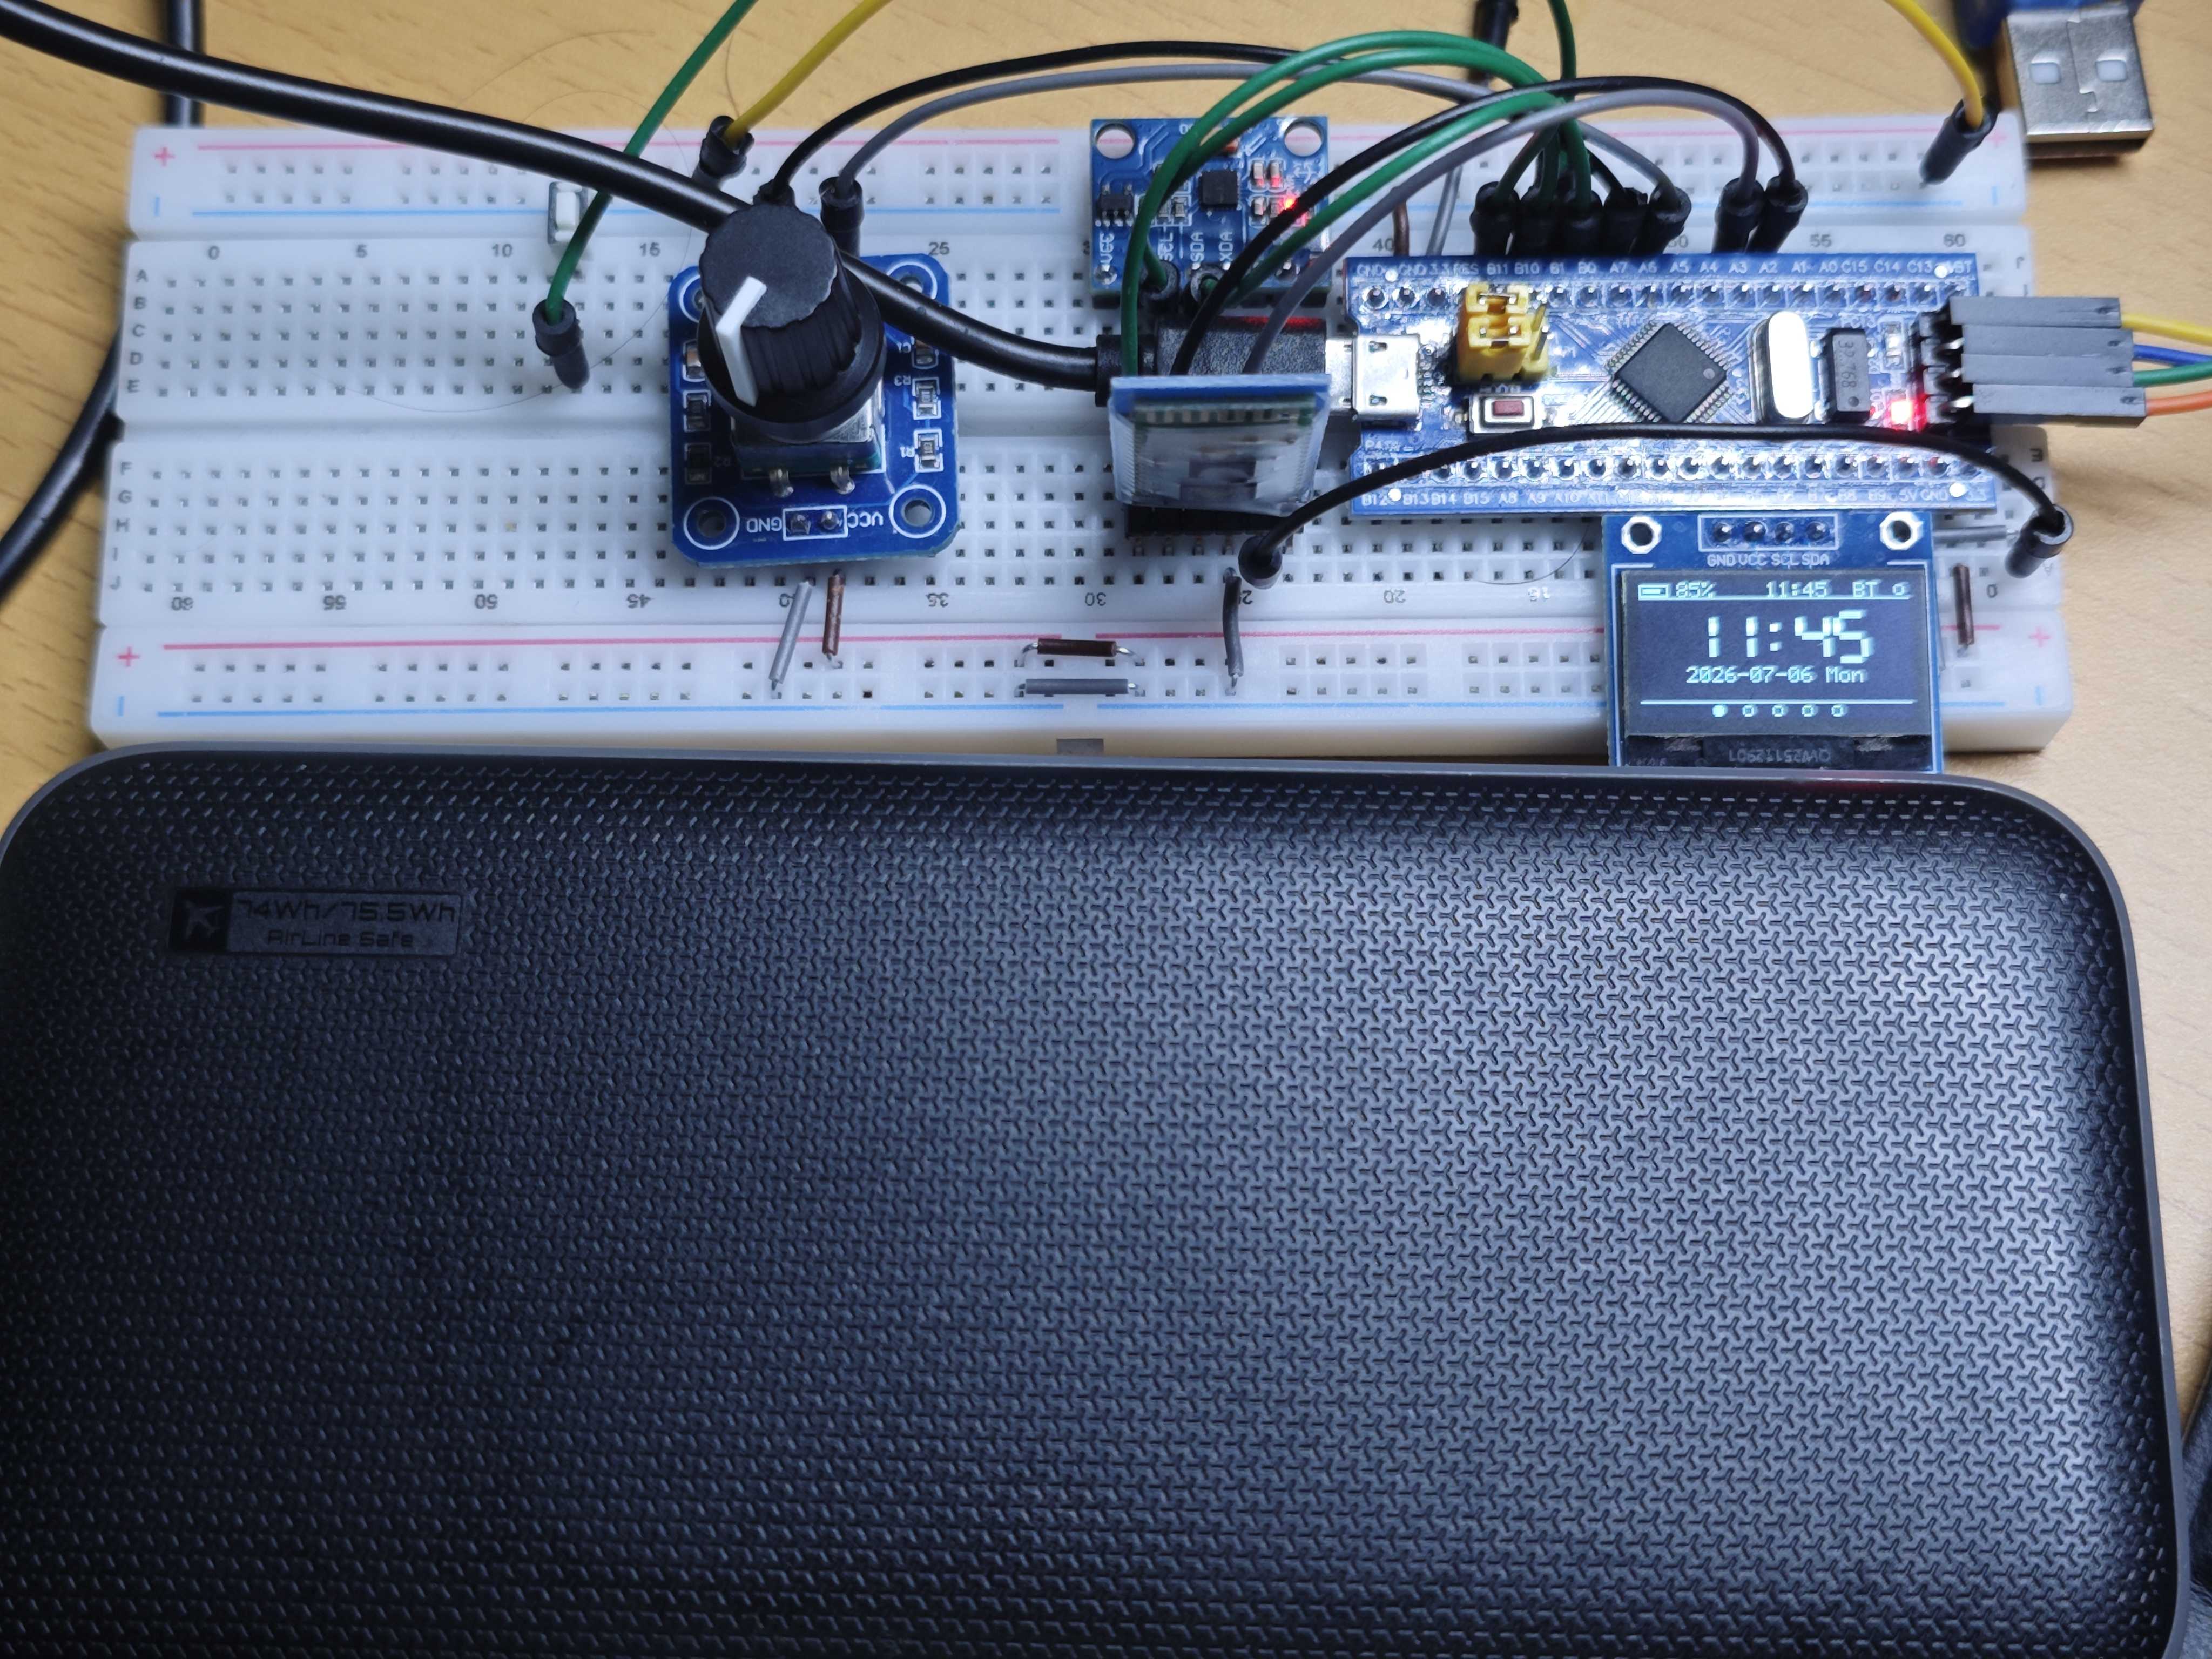
\includegraphics[width=0.82\textwidth]{hardware-wiring.jpg}
  \caption{智能手表实物接线图}
  \label{fig:hardware-wiring}
\end{figure}

主要硬件连接见表~\ref{tab:hardware-pins}。

\begin{table}[H]
  \centering
  \caption{硬件模块与 STM32 引脚分配}
  \label{tab:hardware-pins}
  \small
  \begin{tabularx}{\textwidth}{llp{3.6cm}Y}
    \toprule
    模块 & 接口 & STM32 引脚 & 说明 \\
    \midrule
    SSD1306 OLED & I2C1 & PB6/SCL，PB7/SDA & OLED 地址为 0x3C，供电使用 3.3V \\
    MPU6050 & I2C2 & PB10/SCL，PB11/SDA & AD0 接低电平时地址为 0x68 \\
    HC-05 & USART2 & PA2/TX，PA3/RX，PB0/STATE & 串口参数为 9600 8N1，STATE 用于判断连接状态 \\
    旋转编码器 & GPIO & PA6，PA7 & A/B 相输入，软件消抖和方向判断 \\
    独立按键 & GPIO & PB1 & 替代编码器 SW 引脚，用于返回表盘页 \\
    电源与地 & -- & 3.3V/5V/GND & 各模块共地，按模块要求选择供电电压 \\
    \bottomrule
  \end{tabularx}
\end{table}

HC-05 模块在调试中确认数据模式使用 9600 波特率。STM32 的 PA2 连接 HC-05 RXD，PA3 连接 HC-05 TXD，PB0 读取 HC-05 的 STATE 引脚。Android 手机需要先在系统蓝牙设置中完成 HC-05 配对，再由上位机 App 建立 SPP 连接。

\subsection{软件架构}

STM32 固件位于 \texttt{SmartWatch\_FreeRTOS/}，核心代码按驱动和应用逻辑拆分。主要文件说明见表~\ref{tab:firmware-files}。

\begin{table}[H]
  \centering
  \caption{STM32 固件主要文件}
  \label{tab:firmware-files}
  \begin{tabularx}{\textwidth}{lY}
    \toprule
    文件 & 功能 \\
    \midrule
    \texttt{Core/Src/app\_freertos.c} & 创建 FreeRTOS 任务，维护共享数据和任务同步 \\
    \texttt{Core/Src/smartwatch\_ui.c} & 绘制 OLED 表盘、多页面 UI 和状态指示 \\
    \texttt{Core/Src/oled.c} & SSD1306 初始化、显存刷新和基础绘图函数 \\
    \texttt{Core/Src/mpu6050.c} & MPU6050 初始化、WHO\_AM\_I 检测和数据读取 \\
    \texttt{Core/Src/encoder.c} & 旋转编码器 A/B 相解码、消抖和按键事件处理 \\
    \texttt{Core/Src/step\_counter.c} & 加速度滤波、阈值判断和步数统计 \\
    \texttt{Core/Src/bluetooth.c} & HC-05 串口收发、帧协议解析和状态上报 \\
    \bottomrule
  \end{tabularx}
\end{table}

Android 上位机位于 \texttt{SmartWatch\_AndroidHost/}，采用原生 Java 实现经典蓝牙 SPP 客户端。程序按蓝牙连接、帧协议解析和界面控制三部分组织，便于与 STM32 固件联调。

\subsection{FreeRTOS 任务划分}

本项目将不同实时性需求拆分为独立任务，任务设置见表~\ref{tab:tasks}。共享的手表状态结构体由互斥量保护，显示任务通过二值信号量触发刷新，避免多个任务同时访问 OLED。

\begin{table}[H]
  \centering
  \caption{FreeRTOS 任务划分}
  \label{tab:tasks}
  \begin{tabularx}{\textwidth}{llllY}
    \toprule
    任务 & 优先级 & 栈大小 & 周期 & 功能 \\
    \midrule
    Clock & 4 & 128 & 1 s & 维护软件时钟和运行时间 \\
    Input & 3 & 192 & 10 ms & 轮询旋转编码器和 PB1 按键，更新页面 \\
    Sensor & 3 & 256 & 50 ms & 读取 MPU6050、计算姿态角和步数 \\
    Display & 2 & 384 & 约 100 ms & 根据当前页面刷新 OLED \\
    Bluetooth & 1 & 256 & 50 ms & 解析手机命令，发送状态帧和传感器帧 \\
    \bottomrule
  \end{tabularx}
\end{table}

任务创建的关键代码如下：

\begin{lstlisting}[style=cstyle,caption={FreeRTOS 任务创建代码},label={lst:tasks}]
ok = (xTaskCreate(TaskClock, "clock", 128, NULL, 4, NULL) == pdPASS) ? ok : pdFAIL;
ok = (xTaskCreate(TaskInput, "input", 192, NULL, 3, NULL) == pdPASS) ? ok : pdFAIL;
ok = (xTaskCreate(TaskSensor, "sensor", 256, NULL, 3, NULL) == pdPASS) ? ok : pdFAIL;
ok = (xTaskCreate(TaskDisplay, "display", 384, NULL, 2, NULL) == pdPASS) ? ok : pdFAIL;
ok = (xTaskCreate(TaskBluetooth, "bt", 256, NULL, 1, NULL) == pdPASS) ? ok : pdFAIL;
\end{lstlisting}

\subsection{OLED 页面设计}

OLED 使用 128$\times$64 分辨率的 SSD1306 屏幕。页面采用轻量化布局，主表盘突出显示时间，其余页面分别显示 IMU、步数、蓝牙和设备信息。实物显示效果如图~\ref{fig:oled-pages} 所示。

\begin{figure}[H]
  \centering
  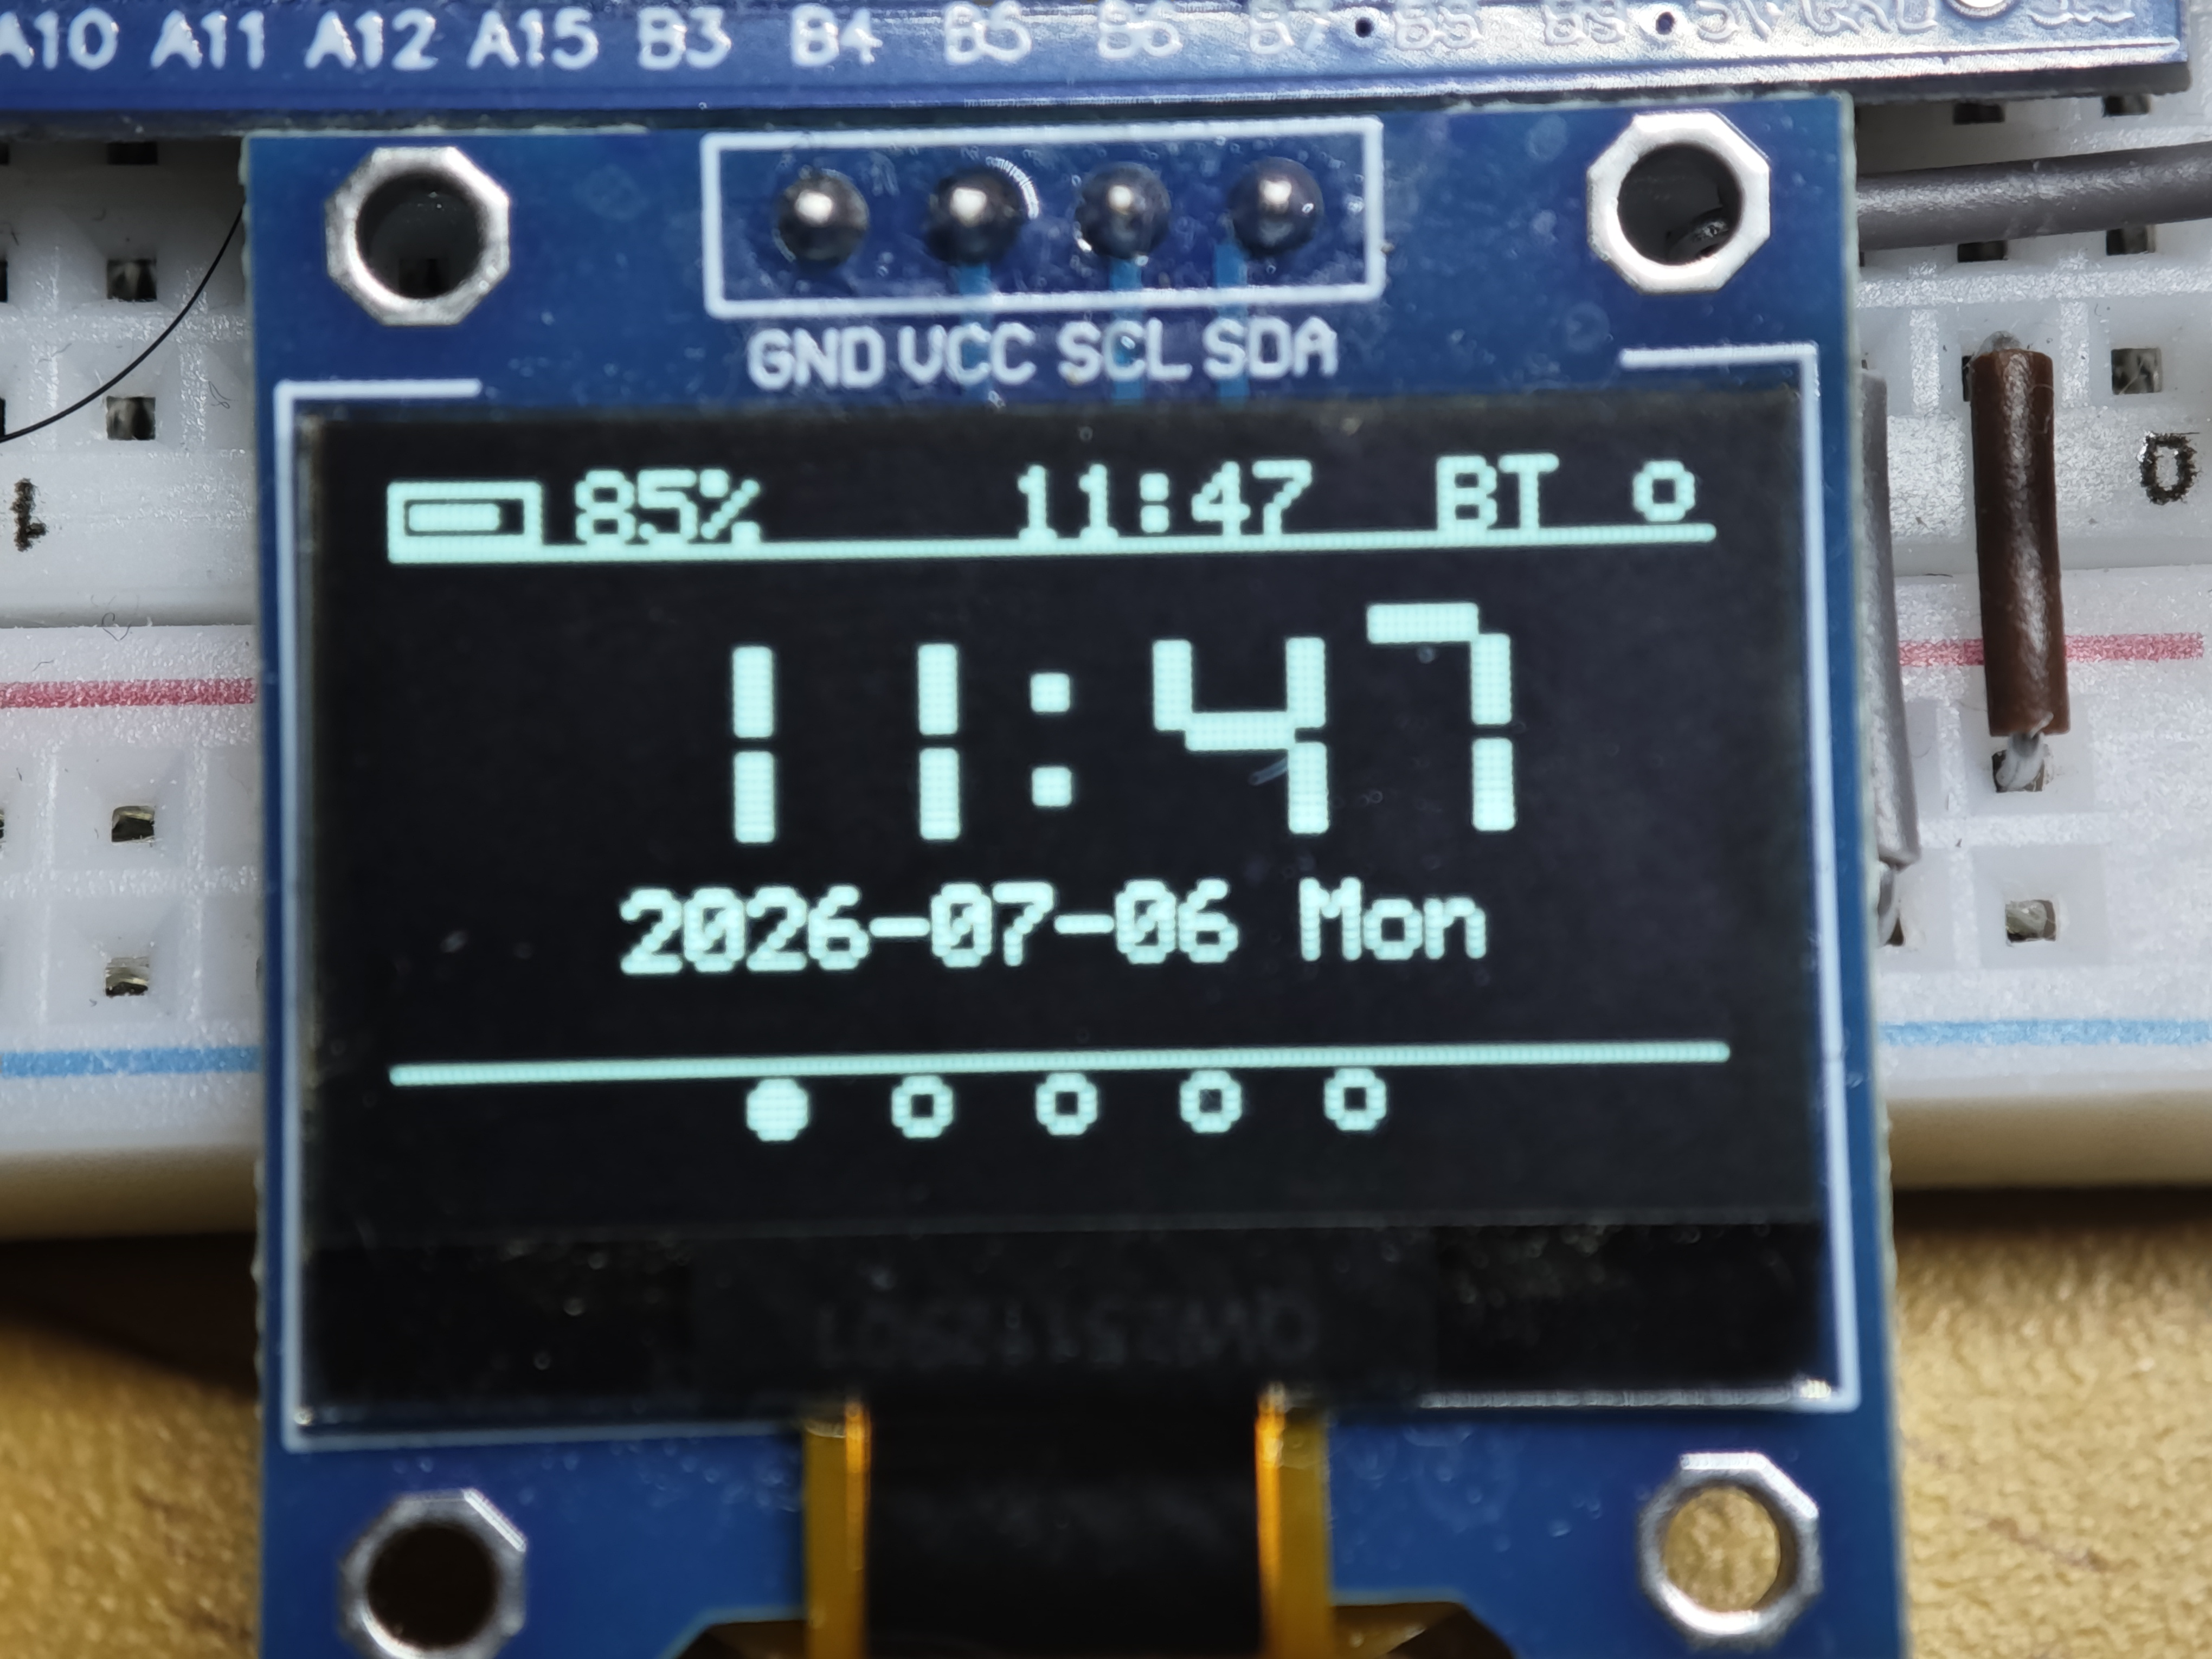
\includegraphics[width=0.76\textwidth]{oled-pages.jpg}
  \caption{OLED 页面显示效果}
  \label{fig:oled-pages}
\end{figure}

前期调试时主表盘曾显示编码器 A/B 状态、方向计数和 MPU 临时状态等调试信息。最终版本已删除这些主表盘调试内容，仅保留时间、日期、状态栏、电量和状态图标等核心显示内容，避免影响验收展示效果。

\subsection{MPU6050 与计步算法}

MPU6050 使用 I2C2 连接，初始化时读取 WHO\_AM\_I 寄存器确认设备在线。传感器任务每 50 ms 读取加速度、角速度和温度。加速度数据用于姿态角估算和基础计步。

计步算法采用加速度模长滤波与阈值判断。程序将三轴加速度转换为合成加速度，使用简单滤波降低抖动，当滤波后的加速度变化超过阈值且满足最小步间隔时累加步数。该方法适合课程演示，能够体现传感器数据处理流程，但精度仍依赖佩戴方式和阈值标定。

\subsection{蓝牙通信与 Android 上位机}

蓝牙通信采用 HC-05 的经典蓝牙 SPP 模式。STM32 与 HC-05 之间通过 USART2 通信，串口参数为 9600 8N1。固件和 Android 上位机使用统一的二进制帧格式，如表~\ref{tab:bt-frame} 所示。

\begin{table}[H]
  \centering
  \caption{蓝牙帧格式}
  \label{tab:bt-frame}
  \begin{tabular}{lllll}
    \toprule
    字段 & 帧头 & 命令 & 长度/数据 & 校验与帧尾 \\
    \midrule
    格式 & 0xAA & CMD & LEN + DATA & CHK + 0x55 \\
    \bottomrule
  \end{tabular}
\end{table}

主要命令见表~\ref{tab:bt-command}。

\begin{table}[H]
  \centering
  \caption{蓝牙命令定义}
  \label{tab:bt-command}
  \begin{tabularx}{\textwidth}{llY}
    \toprule
    命令 & 编号 & 功能 \\
    \midrule
    \texttt{BT\_CMD\_SENSOR\_DATA} & 0x01 & STM32 向手机发送 MPU6050 传感器数据 \\
    \texttt{BT\_CMD\_TIME\_SYNC} & 0x02 & 手机向 STM32 同步时间 \\
    \texttt{BT\_CMD\_ACK} & 0x03 & STM32 返回命令执行结果 \\
    \texttt{BT\_CMD\_STATUS} & 0x04 & STM32 向手机发送当前页面、步数、连接状态等信息 \\
    \texttt{BT\_CMD\_SET\_PAGE} & 0x10 & 手机控制手表切换页面 \\
    \texttt{BT\_CMD\_RESET\_STEPS} & 0x11 & 手机控制手表清零步数 \\
    \texttt{BT\_CMD\_REQUEST\_STATUS} & 0x12 & 手机主动请求状态刷新 \\
    \bottomrule
  \end{tabularx}
\end{table}

Android 上位机界面和蓝牙控制演示分别如图~\ref{fig:android-studio} 与图~\ref{fig:bt-demo} 所示。

\begin{figure}[H]
  \centering
  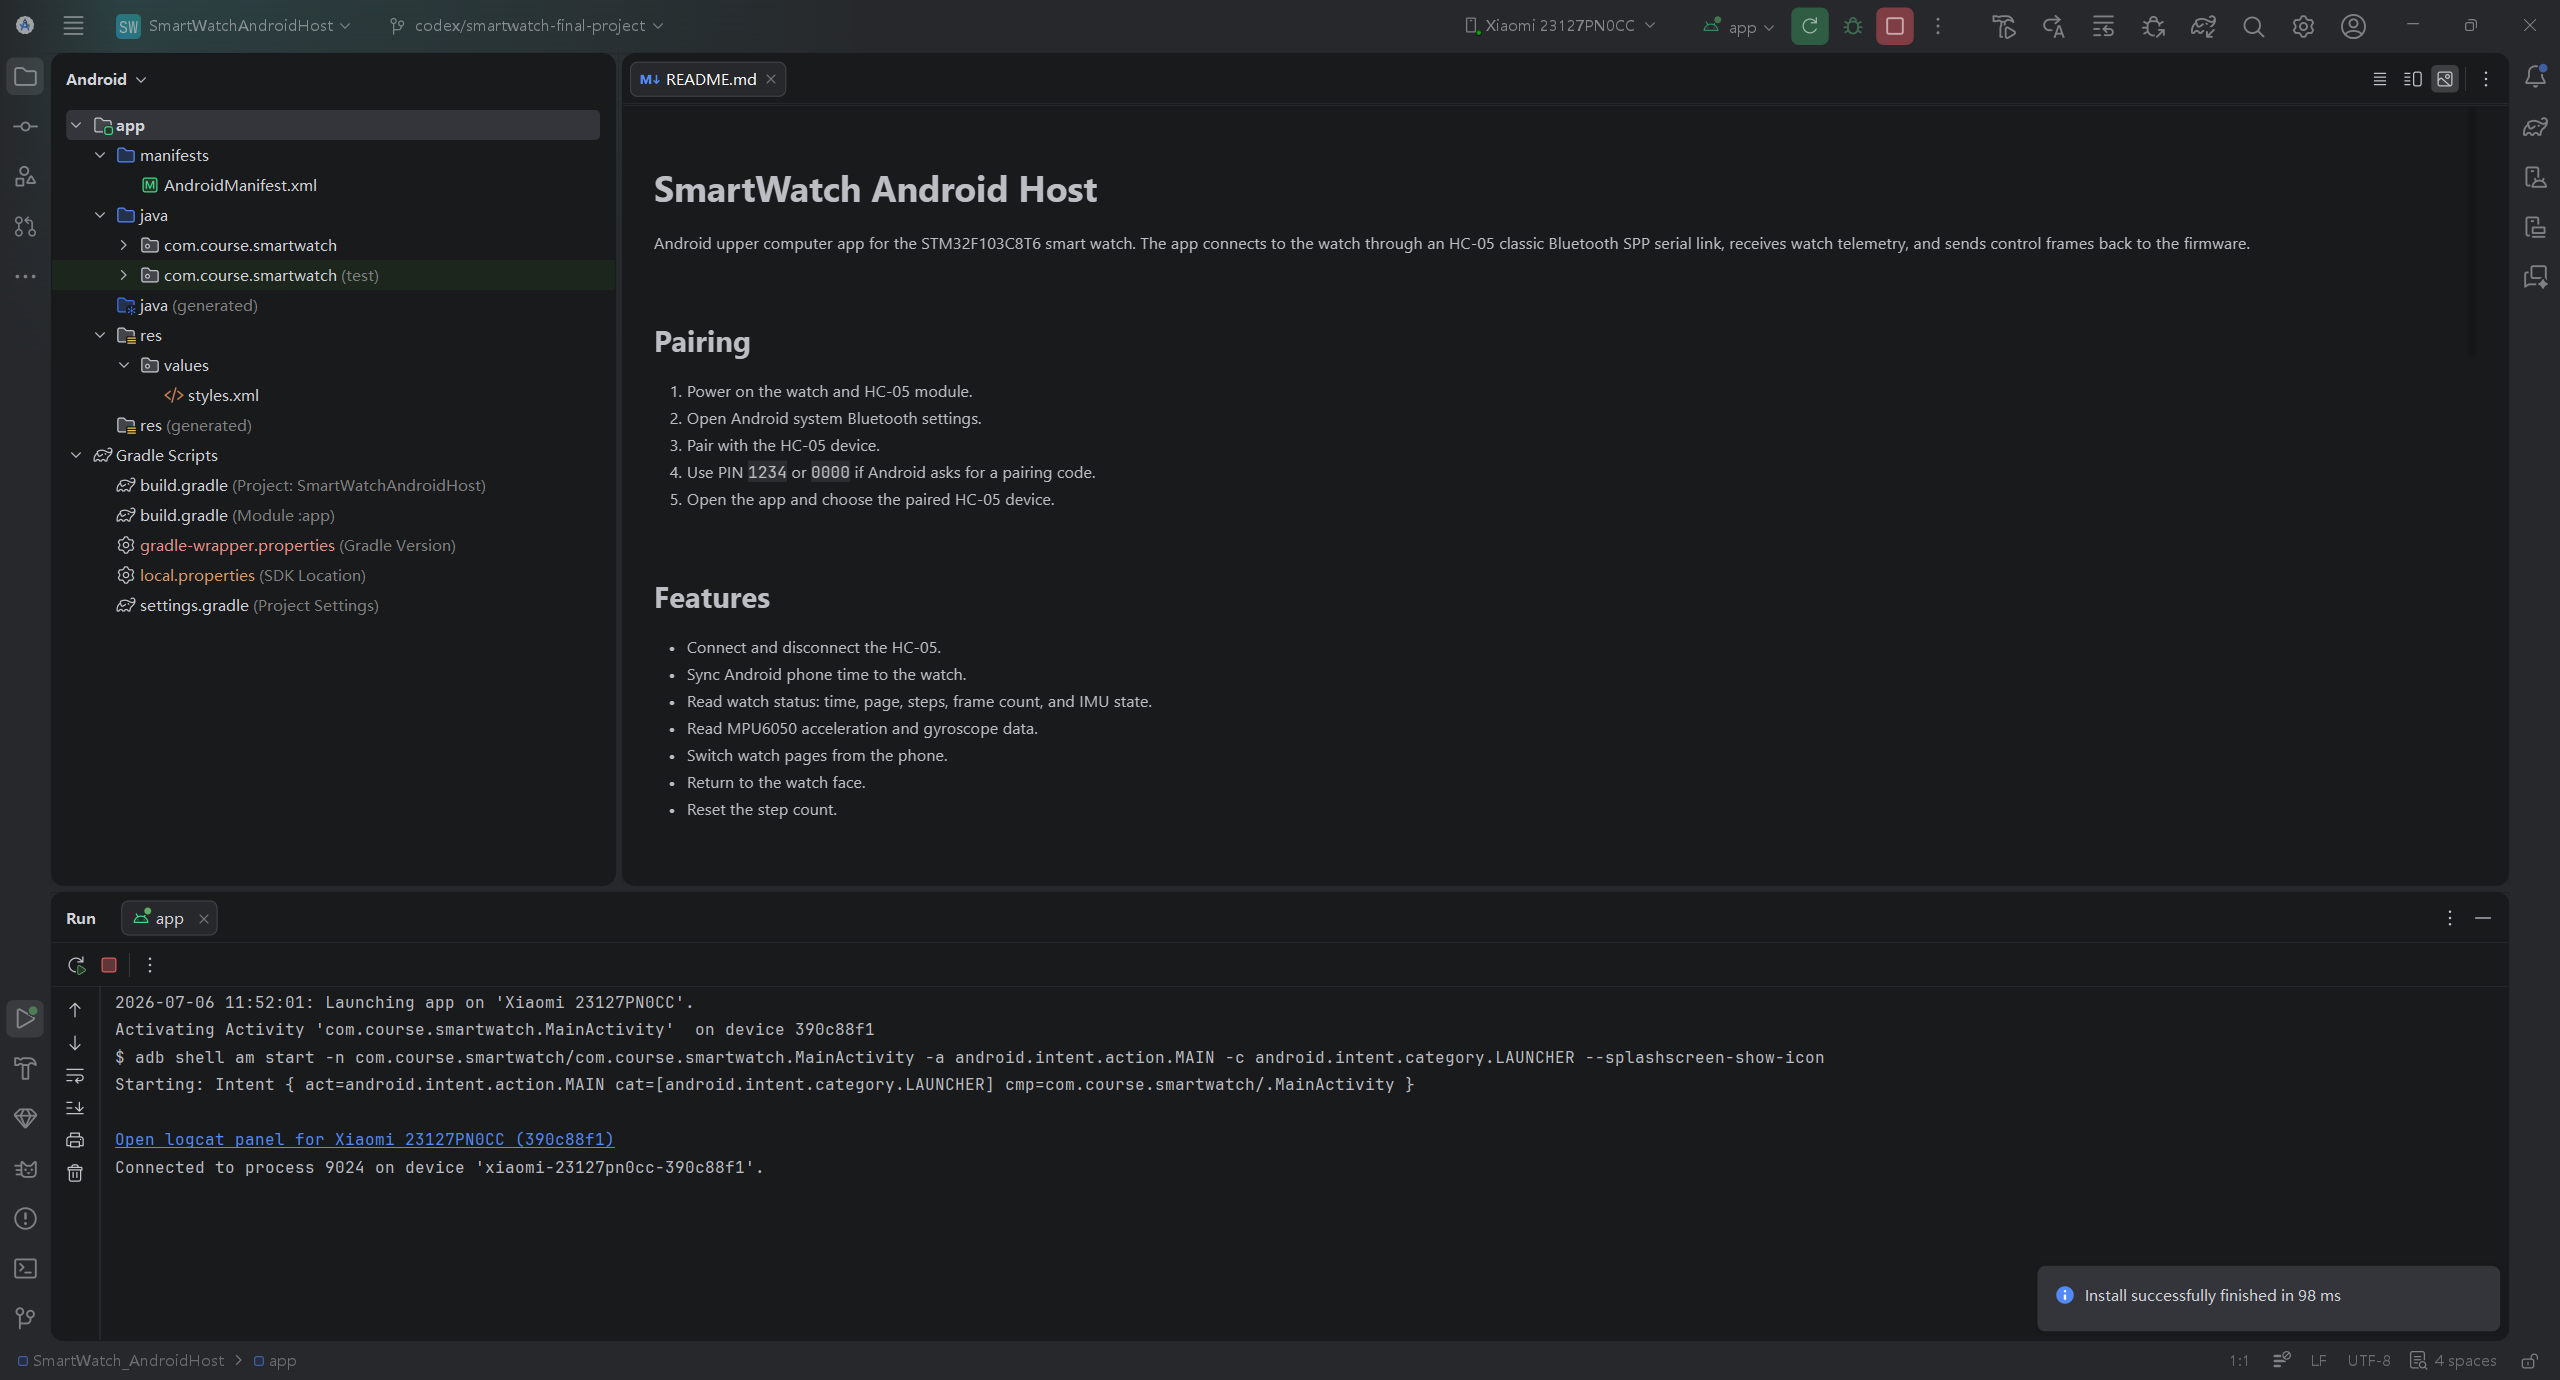
\includegraphics[width=0.9\textwidth]{android-studio.png}
  \caption{Android Studio 上位机工程界面}
  \label{fig:android-studio}
\end{figure}

\begin{figure}[H]
  \centering
  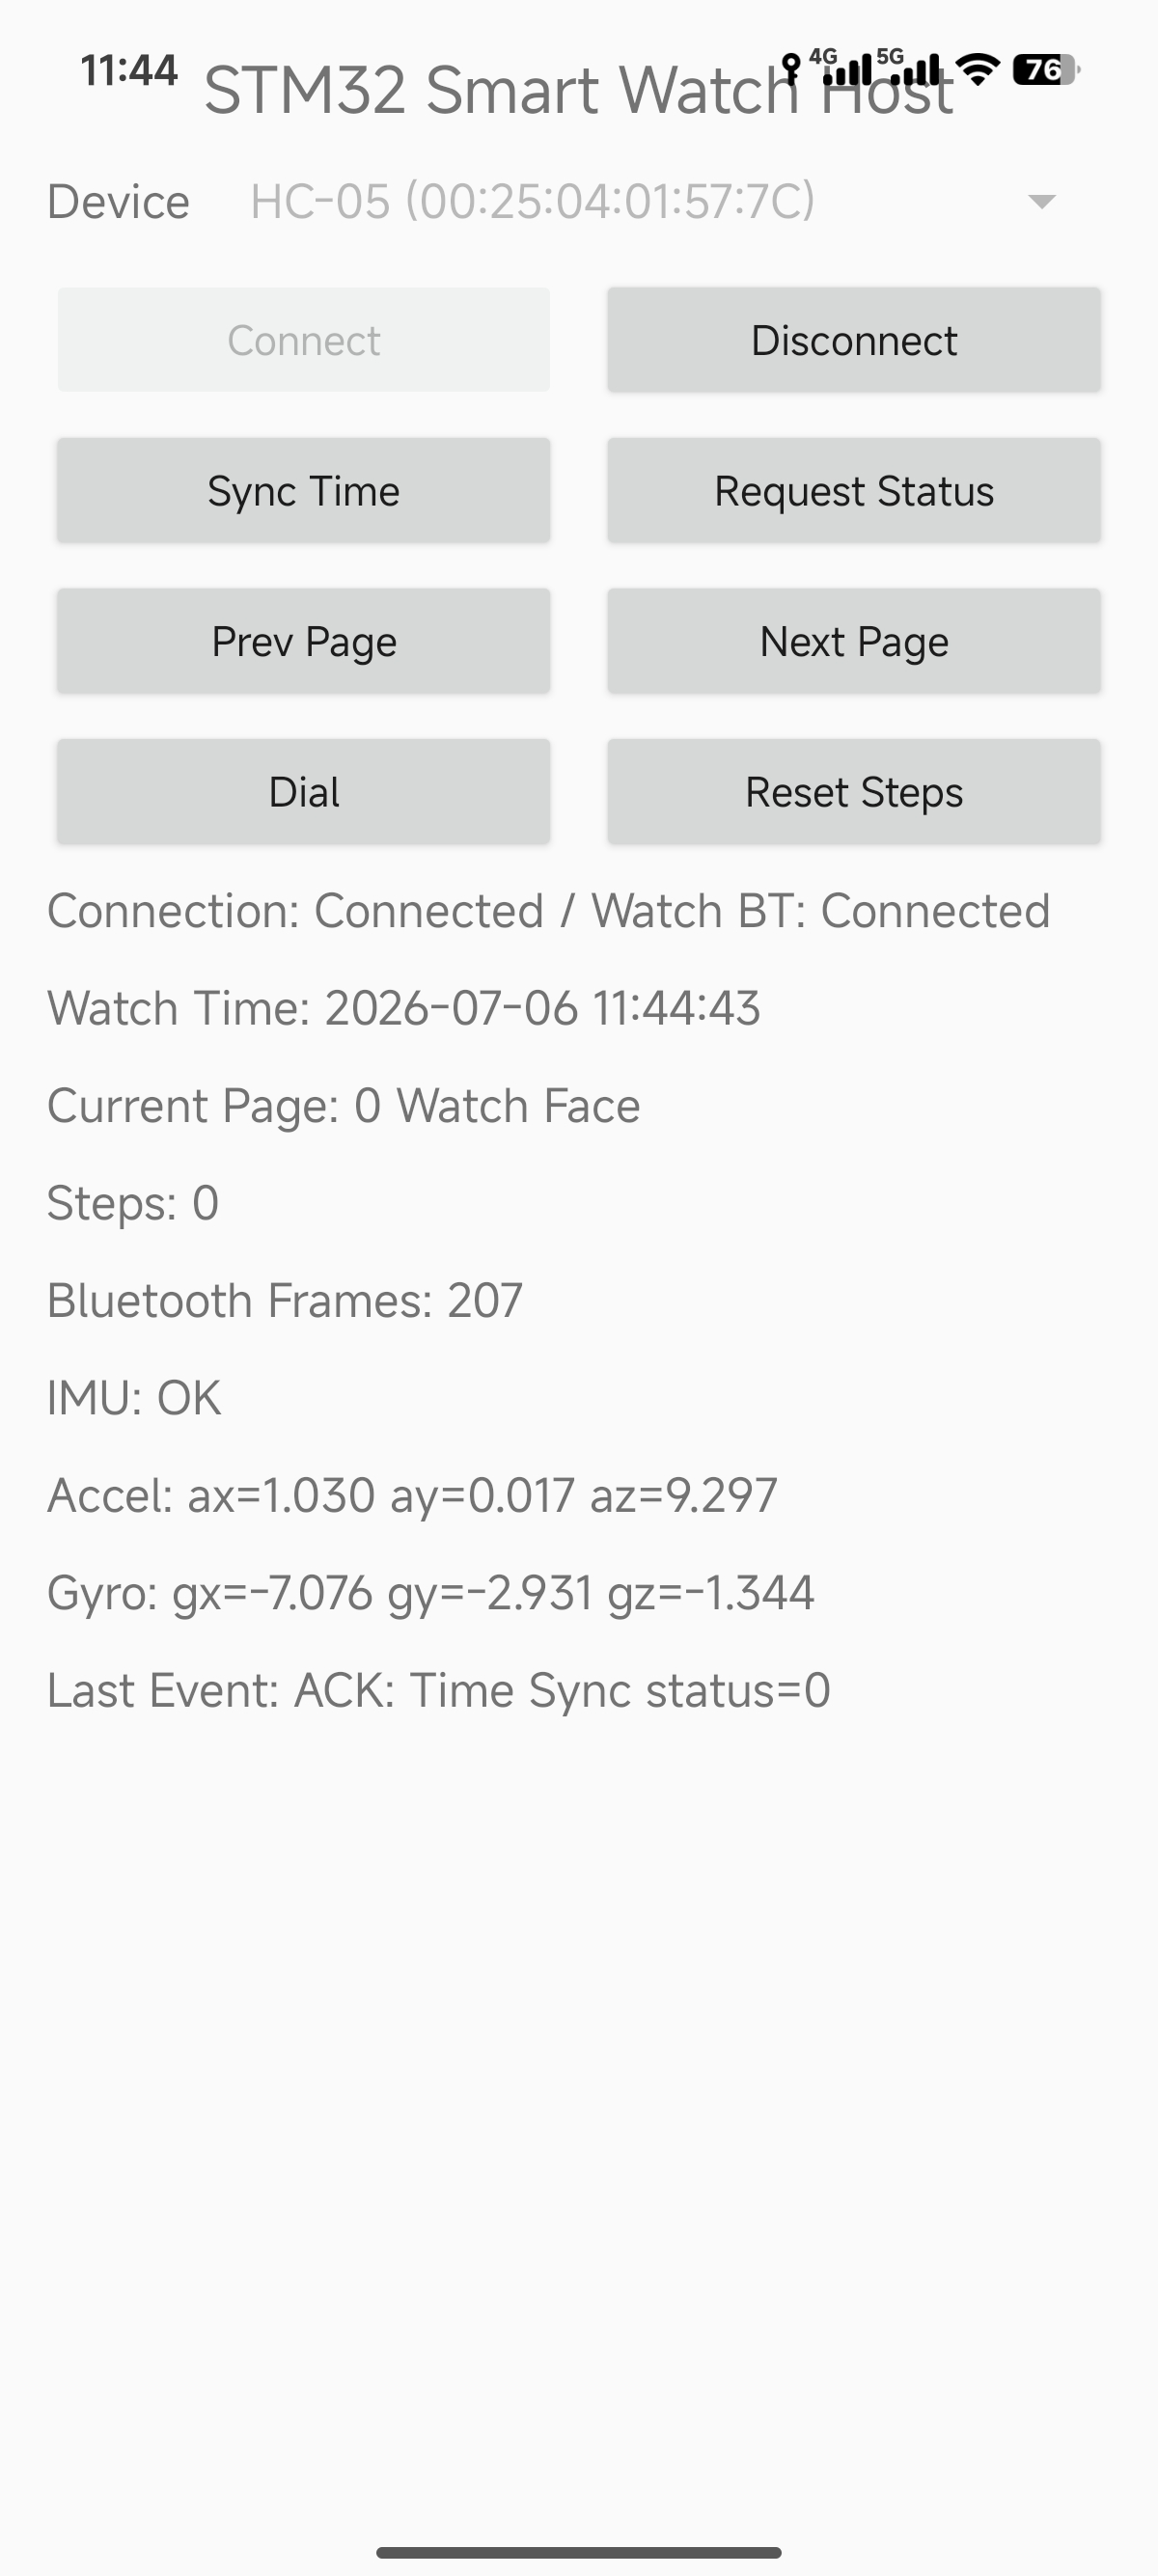
\includegraphics[height=0.66\textheight]{bluetooth-demo.jpg}
  \caption{Android 上位机蓝牙控制演示}
  \label{fig:bt-demo}
\end{figure}

\section{功能展示与测试}

\subsection{测试环境}

测试硬件包括 STM32F103C8T6 最小系统板、SSD1306 OLED、MPU6050、HC-05、旋转编码器、独立按键和 Android 手机。软件环境包括 STM32CubeIDE/CMake/Ninja、TeX Live 2026、Android Studio 和 Android 蓝牙调试环境。

\subsection{功能测试结果}

功能测试结果见表~\ref{tab:test-result}。

\begin{table}[H]
  \centering
  \caption{系统功能测试结果}
  \label{tab:test-result}
  \begin{tabularx}{\textwidth}{lYl}
    \toprule
    测试项目 & 测试方法与现象 & 结果 \\
    \midrule
    OLED 表盘 & 上电后显示主表盘，时间数字、日期和状态栏显示正常 & 通过 \\
    页面切换 & 旋转编码器顺/逆时针切换页面，PB1 返回表盘 & 通过 \\
    MPU6050 & IMU 页面显示加速度、角速度和姿态相关数据 & 通过 \\
    计步 & 摇动或模拟佩戴运动后步数增加，手机端可清零 & 基本通过 \\
    蓝牙连接 & Android 手机配对并连接 HC-05，OLED 蓝牙页显示 CONNECTED & 通过 \\
    手机控制 & 手机端同步时间、切换页面、清零步数和请求状态 & 通过 \\
    数据同步 & 手机端持续接收状态帧和传感器帧，OLED 帧计数增加 & 通过 \\
    \bottomrule
  \end{tabularx}
\end{table}

\subsection{问题与解决过程}

调试过程中遇到的主要问题包括：
\begin{itemize}[leftmargin=2em]
  \item MPU6050 初期无法识别。通过扫描 I2C 地址和读取 WHO\_AM\_I，确认模块地址为 0x68，随后检查接线并将 MPU6050 独立挂到 I2C2，总线稳定后可正常读取。
  \item 旋转编码器初期方向不稳定。通过观察 A/B 电平变化，调整软件解码方式和消抖逻辑，使页面切换恢复为每个有效档位切换一次。
  \item HC-05 初期手机可连接但控制无效。最终确认 HC-05 数据模式为 9600 8N1，将固件、Android 协议和文档统一为 9600 波特率后，手机端控制恢复正常。
  \item 主表盘存在调试信息。最终删除表盘页中的 A/B 相、方向计数和临时 IMU 状态文本，仅保留正式展示信息。
\end{itemize}

\section{物料与成本}

项目物料清单见表~\ref{tab:bom}。价格按常见网购单价估算，实际成本可根据购买渠道调整；手机、电脑和常用工具未计入总成本。

\begin{table}[H]
  \centering
  \caption{项目物料与成本估算}
  \label{tab:bom}
  \small
  \begin{tabularx}{\textwidth}{p{2.7cm}p{3.3cm}rrY}
  \toprule
  物料 & 型号/说明 & 数量 & 单价/元 & 用途 \\
  \midrule
  STM32 最小系统板 & STM32F103C8T6 & 1 & 18.00 & 主控 \\
  OLED 显示屏 & SSD1306 I2C & 1 & 13.00 & 表盘和页面显示 \\
  姿态传感器 & MPU6050 & 1 & 8.00 & 加速度、陀螺仪和计步输入 \\
  蓝牙模块 & HC-05 & 1 & 18.00 & 手机数据同步 \\
  旋转编码器 & EC11 类模块 & 1 & 3.00 & 页面切换 \\
  独立按键 & 轻触按键模块 & 1 & 1.00 & 返回表盘 \\
  面包板/杜邦线 & 若干 & 1 & 10.00 & 模块连接 \\
  ST-LINK 下载器 & ST-LINK/V2 & 1 & 12.00 & 下载和调试 \\
  USB 数据线 & Micro USB/Type-C & 1 & 5.00 & 供电和调试 \\
  \midrule
  \multicolumn{3}{r}{合计} & 88.00 & 不含手机和电脑 \\
  \bottomrule
  \end{tabularx}
\end{table}

\section{个人贡献}

本人在本项目中主要完成以下工作：
\begin{enumerate}[leftmargin=2em]
  \item 根据课程要求分析智能手表功能，确定以 STM32F103C8T6、SSD1306、MPU6050、HC-05 和旋转编码器为核心的方案；
  \item 完成实物接线、模块供电和外设引脚分配，处理 OLED、MPU6050、HC-05 与输入模块的连接问题；
  \item 完成 FreeRTOS 多任务结构设计，将时钟、输入、传感器、显示和蓝牙拆分为独立任务；
  \item 调试 OLED 页面、编码器翻页、PB1 返回表盘、MPU6050 数据读取和计步功能；
  \item 完成 HC-05 与 Android 手机上位机的数据同步和远程控制功能；
  \item 整理 README、检查报告、实物图片和课程设计实验报告。
\end{enumerate}

在开发过程中，个人投入主要集中在硬件连接调试、嵌入式软件开发、蓝牙协议联调和文档整理。由于没有制作 PCB，硬件部分的重点转为保证模块接线稳定、接口说明清晰和功能演示完整。

\section{项目成果与反思}

\subsection{项目成果}

项目已形成一个可现场演示的 STM32 智能手表原型。系统能够稳定显示 OLED 表盘，支持旋转编码器翻页和 PB1 返回表盘；MPU6050 页面能够显示传感器数据；蓝牙页面能够显示连接状态和帧计数；Android 上位机可连接 HC-05 并完成同步时间、切换页面、清零步数、请求状态和读取传感器数据。

从课程设计要求看，项目已完成基本要求，并完成了旋转编码器菜单、蓝牙同步、Android 上位机和计步功能等扩展内容。PCB 部分未完成，但已根据教师允许采用最小系统板的说明，在报告中明确说明替代实现方式。

\subsection{不足与改进方向}

项目仍有以下可改进之处：
\begin{itemize}[leftmargin=2em]
  \item 当前时间由软件时钟维护，断电后不会保持，后续可增加 RTC 或由手机自动同步；
  \item 电量图标目前偏展示性质，后续可增加 ADC 分压采样，实现真实电池电压估算；
  \item 计步算法为基础阈值法，后续可通过更多实测数据标定阈值，降低误计数；
  \item 硬件仍为模块化接线，抗干扰和便携性不如 PCB，后续可绘制正式原理图与 PCB；
  \item Android 上位机界面可继续优化，并打包生成正式 APK 供验收安装。
\end{itemize}

\section{附录}

\subsection{代码清单位置}

完整代码已整理在项目目录中，主要路径如下：
\begin{itemize}[leftmargin=2em]
  \item STM32 固件工程：\texttt{SmartWatch\_FreeRTOS/}
  \item Android 上位机工程：\texttt{SmartWatch\_AndroidHost/}
  \item 课程设计检查报告：\texttt{docs/课程设计项目检查报告.md}
  \item 课程实验报告源码：\texttt{CourseReport/main.tex}
\end{itemize}

\subsection{编译与烧录说明}

STM32 固件可使用 STM32CubeIDE 或 CMake/Ninja 编译。编译通过后，将生成的 ELF 或 HEX 文件使用 ST-LINK 和 STM32CubeProgrammer 烧录到 STM32F103C8T6。Android 上位机使用 Android Studio 打开 \texttt{SmartWatch\_AndroidHost/}，连接 Android 手机后安装调试版本。

\subsection{参考资料}

\begin{enumerate}[leftmargin=2em]
  \item STMicroelectronics，STM32F103x8/xB Datasheet。
  \item STMicroelectronics，STM32Cube HAL Driver Documentation。
  \item FreeRTOS Kernel Documentation。
  \item InvenSense，MPU-6000 and MPU-6050 Product Specification。
  \item SSD1306 OLED Controller Datasheet。
  \item Android Developers，Bluetooth Classic API Documentation。
\end{enumerate}

\end{document}
